\section{Expert Idea Writing and Reviewing}
\label{sec:human_study}
% Now that we have covered the details of how our AI agent generates ideas, we turn to the
% We present human study details in this section, where we introduce the details about our recruited experts, the idea writing, and the idea reviewing. 
In this section, we shift focus to the human branch of idea generation comparison. We present the details of our human study, including information about the recruited experts, the human idea generation task, and the subsequent review process. 


\subsection{Expert Recruitment}

We recruit our expert participants (including for idea writing and reviewing) by sending sign-up forms to several channels, including: 1) the OpenNLP Slack channel with 1426 NLP researchers from 71 institutions (with consent from the channel manager); 2) Twitter (X); 3) Slack channels of various NLP groups by direct communication with the group members; and 4) official chat app of the NAACL 2024 conference. We also conducted in-person recruitment by giving out name cards and wearing T-shirts~\footnote {\url{https://x.com/ChengleiSi/status/1804273510656749649}} with sign-up links at the NAACL 2024 conference as well as various other local NLP social events. Our study % including all recruitment materials 
has been approved by the Stanford IRB (ID 74246). 

We performed screening on all the US participants~\footnote{We have to recruit participants located in the US due to logistical reasons.} based on their provided Google Scholar profiles. We set a minimum requirement of having published at least one paper at a major AI venue.~\footnote{E.g., *ACL, NeurIPS, ICLR, ICML, AAAI.} We reached out to all participants who satisfied this requirement with the consent form and followed up with the annotation documents for those who consented to participate. % Due to logistical constraints, we only considered participants who were physically located in the US during the time of this study to make the payment setups easier. 

In the end, we recruited $N = 49$ experts for writing ideas, and $N = 79$ experts for reviewing ideas. 
Note that 24 out of the 79 reviewers also participated in the idea writing, and we made sure no reviewer would review their own idea. This results in $N = 104$ total participants across the two tasks. 
Each idea writer is asked to write one idea within 10 days and we compensate \$300 for each, with a \$1000 bonus for the top 5 ideas as scored by the expert reviewers. 
Each idea reviewer is assigned 2 to 7 ideas to review and we collected $N = 298$ unique reviews in total. 
They are given one week to finish the reviews and we compensated \$25 for each review written by the idea reviewers. 

\subsection{Expert Qualifications}


\begin{wrapfigure}{r}{0.4\textwidth} % 'r' for right, 'l' for left
    \centering
    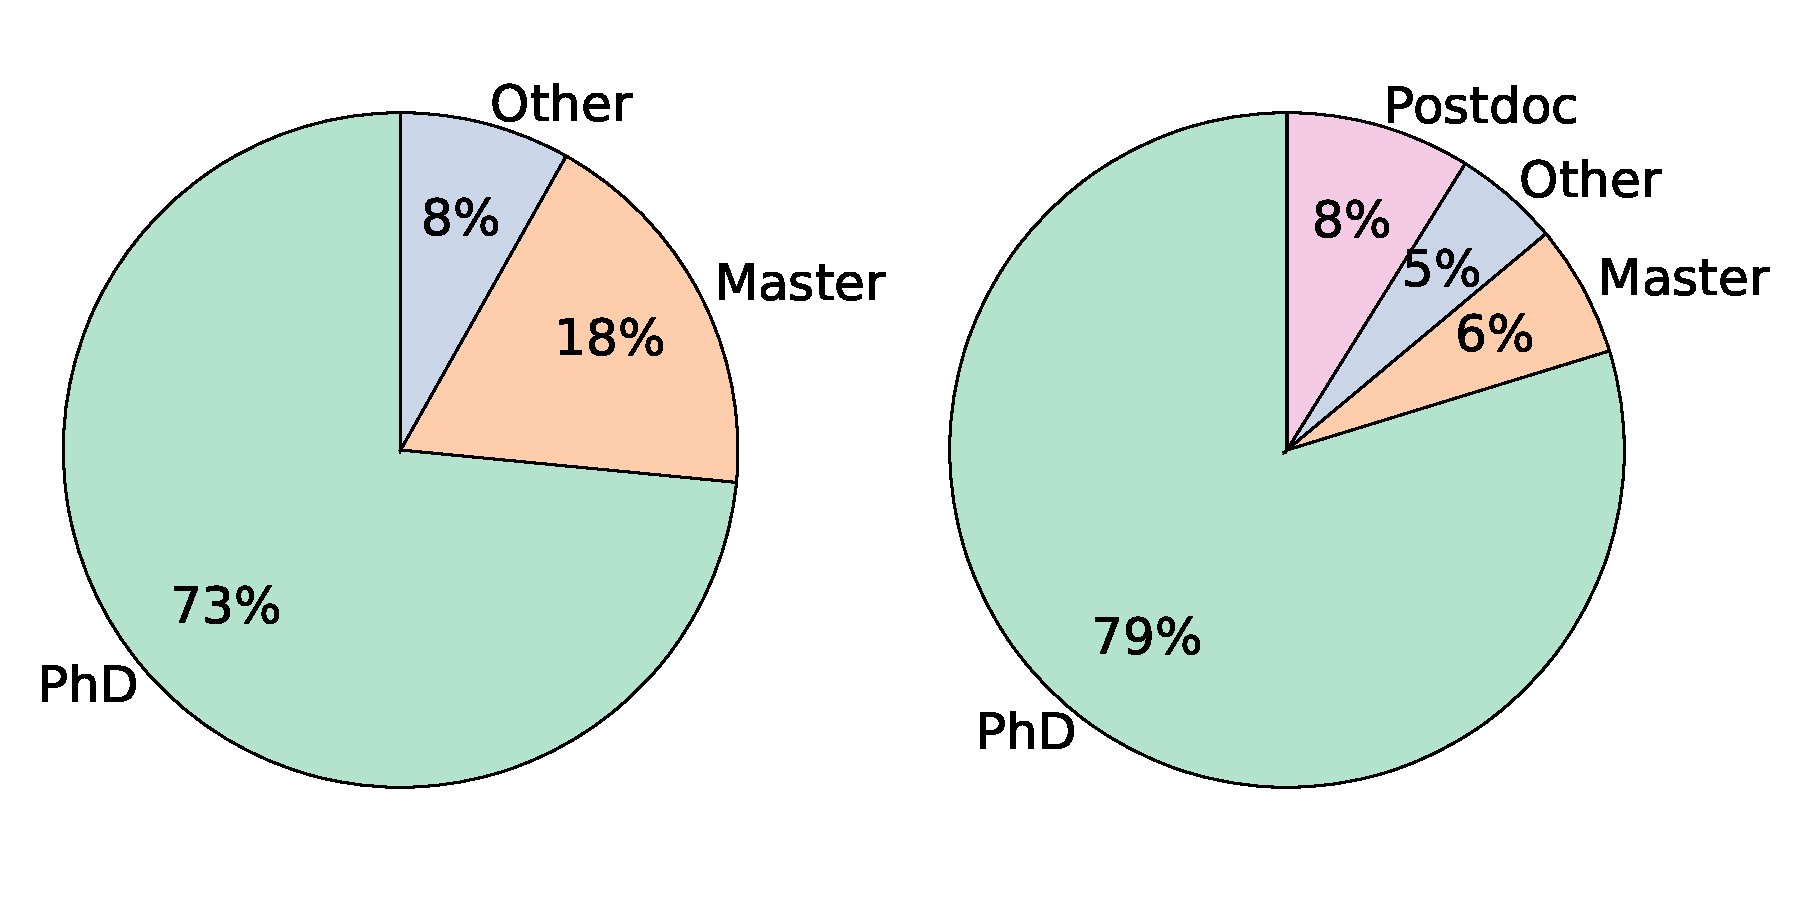
\includegraphics[trim=0 0 0 0,clip,width=0.4\textwidth]{figures/participant_pie.pdf}
    \caption{Positions of our idea writer (left) and reviewer (right) participants.}
    \label{fig:participant_pie}
    % \vspace{-0.1cm}
\end{wrapfigure}



% \textbf{Idea Writers} 
Our pool of participants is highly qualified and diverse. The 49 idea writers come from 26 different institutions (Table~\ref{table:idea_participants_institution}) and the majority of them are current PhD students (Figure~\ref{fig:participant_pie} left).  
The 79 reviewers come from 32 institutions (Table~\ref{table:reviewer_institution}) and are mostly PhD students and Postdocs (Figure~\ref{fig:participant_pie} right). 
%
We use their Google Scholar profiles to extract several proxy metrics, including the number of papers, citations, h-index, and i10-index at the time of their submission. Table~\ref{table:merged_profile} shows that our idea writers have an average of 12 papers and 477 citations, while every reviewer has published at least two papers and has an average citation of 635 and h-index of 7. 
Moreover, based on their survey responses, 72 out of the 79 reviewers have previously reviewed for major AI conferences or journals. 
These statistics indicate that our participants are highly qualified and have substantial research experience.~\footnote{Detailed breakdown of participant positions is in Appendix~\ref{sec:participant_positions}.} 
% Table~\ref{table:reviewer_position} shows that the majority of these reviewers are current PhD students or Postdocs, and Table~\ref{table:reviewer_profile} shows that every reviewer has published at least two papers and has an average citation of 635 and h-index of 7. 
% Based on their survey responses, 72 out of the 79 reviewers have previously reviewed for major AI conferences or journals. 


\begin{table}[t]
\small
\centering
\begin{tabular}{l c c c c c | c c c c c} 
 \hline
 & \multicolumn{5}{c|}{Idea Writing Participants (N=49)} & \multicolumn{5}{c}{Idea Reviewing Participants (N=79)} \\ 
 \hline
 Metric & Mean & Median & Min & Max & SD & Mean & Median & Min & Max & SD \\ 
 \hline
papers & 12 & 10 &  2 & 52 & 9 & 15 & 13 & 2 & 52 & 10 \\ 
citations & 477 & 125 & 2 & 4553 & 861 & 635 & 327 & 0 & 7276 & 989 \\
h-index & 5 & 4 & 1 & 21 & 4 & 7 & 7 & 0 & 21 & 4 \\
i10-index & 5 & 4 & 0 & 32 & 6 & 7 & 5 & 0 & 32 & 6 \\
 \hline
\end{tabular}
\caption{Research profile metrics of the idea writing and reviewing participants. Data are extracted from Google Scholar at the time of idea or review submission.}
\label{table:merged_profile}
\end{table}



% \textbf{Annotation}
% Each expert is instructed to choose one of the seven specified topics and write one idea on it within a week, following the given template in the annotation document.  
% We included an honor code statement to ask the participants to not use any AI tools in their idea writing. 
% We collected $N = 50$ ideas originally and manually checked all of them for quality control. We filtered out one of them as being essentially a paraphrase of an existing paper's abstract~\footnote{We compensated the participant nevertheless, but excluded them for the review task.}. We keep the remaining $N = 49$ human ideas for the human-AI comparison and show the topic distribution in Table~\ref{table:topic_distribution}. For the \texttt{AI Ideas} and \texttt{AI Ideas + Human Rerank} conditions, we also generate $N = 49$ ideas to match the same topic distribution for a fair comparison across conditions. 


% \begin{table}[ht]
% \centering
% \begin{tabular}{c c} 
%  \hline
%  Position & Count \\ 
%  \hline
% Postdoc & 1 \\
% PhD & 36 \\
% Master & 9 \\
% Undergraduate & 1 \\
% Research Scientist & 1 \\
% Machine Learning Engineer & 1 \\
%  \hline
% \end{tabular}
% \caption{Positions of the 49 idea writing participants.}
% \label{table:idea_participants_position}
% \end{table}


% \begin{table}[ht]
% \centering
% \begin{tabular}{l c c c c c} 
%  \hline
%  Metric & Mean & Median & Min & Max & SD \\ 
%  \hline
% papers & 12 & 10 &  2 & 52 & 9\\ 
% citations & 477 & 125 & 2 & 4553 & 861 \\
% h-index & 5 & 4 & 1 & 21 & 4 \\
% i10-index & 5 & 4 & 0 & 32 & 6 \\
%  \hline
% \end{tabular}
% \caption{Proxy metrics on the research profiles of the 49 idea writing participants. All data are extracted from Google Scholar at the time of their idea submission.}
% \label{table:idea_participants_profile}
% \end{table}


% \textbf{Participant Statistics} 
% Our pool of participants is highly qualified and diverse. They come from 26 different institutions (Table~\ref{table:idea_participants_institution}) and the majority of them are current PhD students (Table~\ref{table:idea_participants_position}).  
% We use their Google Scholar profiles to extract several proxy metrics, including the number of papers, citations, h-index, and i10-index at the time of their idea submission. Table~\ref{table:idea_participants_profile} shows that our idea writers have an average of 12 papers and 477 citations, indicating substantial research experiences.  



\begin{table}[t]
\centering
\small 
\begin{tabular}{l c c c c c} 
 \hline
 Metric & Mean & Median & Min & Max & SD \\ 
 \hline
 \texttt{Human} Ideas  \\
 Familiarity (1-5) & 3.7 & 4.0 & 1.0 & 5.0 & 1.0 \\
 Difficulty (1-5) & 3.0 & 3.0 & 1.0 & 5.0 & 0.7 \\
 Time (Hours) & 5.5 & 5.0 & 2.0 & 15.0 & 2.7 \\
 Length (Words) & 901.7 & 876.0 & 444.0 & 1704.0 & 253.5 \\
 \hline
 \texttt{AI} Ideas \\
 Length (Words) & 1186.3 & 1158.0 & 706.0 & 1745.0 & 233.7 \\
 \hline 
 \texttt{AI + Human Rerank} Ideas \\
 Length (Words) & 1174.0 & 1166.0 & 706.0 & 1708.0 & 211.0 \\
 \hline
\end{tabular}
\caption{Statistics of the 49 ideas from each condition.}
\label{table:idea_statistics}
\end{table}



\begin{wraptable}{r}{0.35\textwidth} % 'r' aligns the table to the right, and the width is 45% of the text width.
\centering
\small
\begin{tabular}{l c} 
 \hline
 Topic & Count \\ 
 \hline
 Bias & 4 \\
 Coding & 9 \\
 Safety & 5 \\
 Multilingual & 10 \\
 Factuality & 11 \\
 Math & 4 \\
 Uncertainty & 6 \\
 \hline 
 Total & 49 \\
 \hline
\end{tabular}
\caption{Idea topic distribution.}
\label{table:topic_distribution}
\vspace{-0.2cm}
\end{wraptable}



\subsection{Idea Writing}


We report statistics of our idea writers' ideas to measure their quality. 
As shown in Table~\ref{table:idea_statistics}, idea writers indicate a moderately high familiarity with their selected topic (3.7 on a 1 to 5 scale), and indicate the task as moderately difficult (3 on a 1 to 5 scale). They spent an average of 5.5 hours on the task and their ideas are 902 words long on average. These indicate that participants are putting substantial effort into this task.~\footnote{See Appendix~\ref{sec:idea_quality_control} for more details on the quality control of human ideas.} 
We also show the distribution of their selected topics in Table~\ref{table:topic_distribution}. 
% and ranked their submitted idea as top $43.4\%$ among all their published ideas. 
% We also compute the length (word count) of all ideas across the three conditions after the style standardization. 





% \begin{table}[h]
% \small 
% \centering
% \begin{minipage}[b]{0.45\textwidth}
% \centering
% \begin{tabular}{l c c c c c} 
%  \hline
%  Metric & Mean & Median & Min & Max & SD \\ 
%  \hline
% papers & 12 & 10 &  2 & 52 & 9\\ 
% citations & 477 & 125 & 2 & 4553 & 861 \\
% h-index & 5 & 4 & 1 & 21 & 4 \\
% i10-index & 5 & 4 & 0 & 32 & 6 \\
%  \hline
% \end{tabular}
% \caption{Proxy metrics on the research profiles of the 49 idea writing participants. All data are extracted from Google Scholar at the time of their idea submission.}
% \label{table:idea_participants_profile}
% \end{minipage}
% \hspace{0.05\textwidth}
% \begin{minipage}[b]{0.45\textwidth}
% \centering
% \begin{tabular}{l c c c c c} 
%  \hline
%  Metric & Mean & Median & Min & Max & SD \\ 
%  \hline
% papers & 15 & 13 & 2 & 52 & 10 \\ 
% citations & 635 & 327 & 0 & 7276 & 989 \\
% h-index & 7 & 7 & 0 & 21 & 4 \\
% i10-index & 7 & 5 & 0 & 32 & 6 \\
%  \hline
% \end{tabular}
% \caption{Statistics of the research profiles of the 79 reviewers. Data are extracted from Google Scholar at the time of their review submission.}
% \label{table:reviewer_profile}
% \end{minipage}
% \end{table}





% \begin{table}[t]
% \small
% \centering
% \begin{minipage}[b]{0.45\textwidth}
% \centering
% \begin{tabular}{c c} 
%  \hline
%  Position & Count \\ 
%  \hline
% Postdoc & 7 \\
% PhD & 63 \\
% Master & 5 \\
% Research Scientist & 3 \\
% Machine Learning Engineer & 1 \\
%  \hline
% \end{tabular}
% \caption{Positions of the 79 reviewer participants.}
% \label{table:reviewer_position}
% \end{minipage}
% \hspace{0.05\textwidth}
% \begin{minipage}[b]{0.45\textwidth}
% \centering
% \begin{tabular}{l c c c c c} 
%  \hline
%  Metric & Mean & Median & Min & Max & SD \\ 
%  \hline
% papers & 15 & 13 & 2 & 52 & 10 \\ 
% citations & 635 & 327 & 0 & 7276 & 989 \\
% h-index & 7 & 7 & 0 & 21 & 4 \\
% i10-index & 7 & 5 & 0 & 32 & 6 \\
%  \hline
% \end{tabular}
% \caption{Statistics of the research profiles of the 79 reviewers. Data are extracted from Google Scholar at the time of their review submission.}
% \label{table:reviewer_profile}
% \end{minipage}
% \end{table}



% \begin{table}[ht]
% \centering
% \small 
% \begin{minipage}{0.6\textwidth}
% \centering
% \begin{tabular}{l c c c c c} 
%  \hline
%  Metric & Mean & Median & Min & Max & SD \\ 
%  \hline
%  \texttt{Human}   \\
%  Familiarity (1-5) & 3.7 & 4.0 & 1.0 & 5.0 & 1.0 \\
%  Difficulty (1-5) & 3.0 & 3.0 & 1.0 & 5.0 & 0.7 \\
%  Time (Hours) & 5.5 & 5.0 & 2.0 & 15.0 & 2.7 \\
%  Length (Words) & 901.7 & 876.0 & 444.0 & 1704.0 & 253.5 \\
%  \hline
%  \texttt{AI} \\
%  Length (Words) & 1186.3 & 1158.0 & 706.0 & 1745.0 & 233.7 \\
%  \hline 
%  \texttt{AI + Human Rerank} \\
%  Length (Words) & 1174.0 & 1166.0 & 706.0 & 1708.0 & 211.0 \\
%  \hline
% \end{tabular}
% \caption{Statistics of the 49 ideas from each condition.}
% \label{table:idea_statistics}
% \end{minipage}%
% \hfill
% \begin{minipage}{0.35\textwidth}
% \centering
% \begin{tabular}{l c} 
%  \hline
%  Topic & Count \\ 
%  \hline
%  Bias & 4 \\
%  Coding & 9 \\
%  Safety & 5 \\
%  Multilingual & 10 \\
%  Factuality & 11 \\
%  Math & 4 \\
%  Uncertainty & 6 \\
%  \hline 
%  Total & 49 \\
%  \hline
% \end{tabular}
% \caption{Number of ideas for each topic.}
% \label{table:topic_distribution}
% \end{minipage}
% \end{table}



% \begin{table}[ht]
% \centering
% \small 
% \begin{tabular}{l c c c c c} 
%  \hline
%  Metric & Mean & Median & Min & Max & SD \\ 
%  \hline
%  \texttt{Human} Ideas  \\
%  Familiarity (1-5) & 3.7 & 4.0 & 1.0 & 5.0 & 1.0 \\
%  Difficulty (1-5) & 3.0 & 3.0 & 1.0 & 5.0 & 0.7 \\
% Time (Hours) & 5.5 & 5.0 & 2.0 & 15.0 & 2.7 \\
% % Self-Rank (Top k\%) & 43 & 5 & 90 & 20.3 \\
% Length (Words) & 901.7 & 876.0 & 444.0 & 1704.0 & 253.5 \\
% \hline
% \texttt{AI} Ideas \\
% Length (Words) & 1186.3 & 1158.0 & 706.0 & 1745.0 & 233.7 \\
% \hline 
% \texttt{AI + Human Rerank} Ideas \\
% Length (Words) & 1174.0 & 1166.0 & 706.0 & 1708.0 & 211.0 \\
%  \hline
% \end{tabular}
% \caption{Statistics of the 49 ideas from each condition.}
% \label{table:idea_statistics}
% \end{table}


% \begin{wraptable}{r}{0.4\textwidth}
% \centering
% \small  % Reduce the font size
% \begin{tabular}{l c} 
%  \hline
%  Topic & Count \\ 
%  \hline
%  Bias & 4 \\
%  Coding & 9 \\
%  Safety & 5 \\
%  Multilingual & 10 \\
%  Factuality & 11 \\
%  Math & 4 \\
%  Uncertainty & 6 \\
%  \hline 
%  Total & 49 \\
%  \hline
% \end{tabular}
% \caption{Number of ideas for each topic.}
% \label{table:topic_distribution}
% \end{wraptable}


% \subsection{Style Standardization of All Ideas}

% To avoid the potential confounder that reviewers might pick up on the style differences between the AI ideas and human ideas, we developed a style standardization module to ask an LLM to convert all ideas into the same writing and formatting style without changing the original content.
% We conducted a small-scale human study with five LLM researchers and they achieved 50\% accuracy on the task of distinguishing AI and human ideas after this style standardization. The author of this paper also manually checked all converted writings to ensure all contents of the original ideas are preserved. 
% We present the full prompt used in Appendix~\ref{sec:style_transfer_prompt}.

% \subsection{Expert Reviewing}



\subsection{Idea Reviewing}

\begin{wraptable}{r}{0.45\textwidth}
\centering
\small  
\begin{tabular}{l c c c c} 
 \hline
 Metric & Mean & Min & Max & SD \\ 
 \hline
\# Reviews & 3.8 & 2.0 & 7.0 & 1.3 \\
\# Conditions & 2.5 & 2.0 & 3.0 & 0.5 \\
\# Topics & 1.5 & 1.0 & 3.0 & 0.6 \\
 \hline
\end{tabular}
\caption{Statistics of the review assignment.}
\label{table:reviewer_assignment}
\end{wraptable}


\textbf{Review Assignment}
We let all reviewer participants select their top two preferred topics as well as their preferred reviewing load (from 2 to 7). 
We then randomly assign them to ideas within their selected topics and all ideas are anonymized. 
In the assignment, we balance the number of ideas from each condition for each reviewer and ensure that each reviewer gets at least one human idea and one AI idea. 
Every idea is reviewed by 2 to 4 different reviewers. 
% We anonymize all ideas and randomize the ordering when sending the list of review forms to the reviewers to ensure that all reviewers are blind to the identity of the ideas. 
We also avoid assigning ideas written by authors from the same institution to avoid any potential contamination. 
Table~\ref{table:reviewer_assignment} shows that each reviewer wrote an average of 3.8 reviews from 2 or 3 conditions, across 1 to 3 topics. 




% \textbf{Participant Statistics}
% We recruited a pool of diverse and highly qualified reviewers. Table~\ref{table:reviewer_institution} lists the 32 institutions that these reviewers come from. Table~\ref{table:reviewer_position} shows that the majority of these reviewers are current PhD students or Postdocs, and Table~\ref{table:reviewer_profile} shows that every reviewer has published at least two papers and has an average citation of 635 and h-index of 7. 
% Based on their survey responses, 72 out of the 79 reviewers have previously reviewed for major AI conferences or journals. 


% \textbf{Review Form} We developed a review form similar to AI conference reviewing (e.g., ACL and ICLR). The beginning of the review form includes a pre-survey asking for participant consent, agreement on not to use AI to write reviews,  their familiarity with the selected topic, and their prior review experience. We then present the anonymized idea and ask the following question:
%  \begin{enumerate}[nolistsep]
%     \item Novelty: Score (1 - 10) and Free-Text Rationale 
%     \item Excitement: Score (1 - 10) and Free-Text Rationale 
%     \item Feasibility: Score (1 - 10) and Free-Text Rationale 
%     \item Expected Effectiveness: Score (1 - 10) and Free-Text Rationale 
%     \item Overall: Score (1 - 10) and Free-Text Rationale 
%     \item Post-Survey: Confidence (1 - 5) and Time Spent 
%  \end{enumerate}

 
\textbf{Review Quality Check} 
Apart from ensuring reviewer qualifications, we also compute statistics to measure the quality of the reviews in Table~\ref{table:review_stats}.
On average, the reviewers indicated a familiarity of 3.7 (out of 5) in their selected topic and a confidence of 3.7 (out of 5) in their reviews. This is comparable with the 1.2K ICLR 2024 submissions related to language models, where the reviewers also have an average confidence of 3.7 out of 5. Moreover, reviewers spent an average of 32 minutes on each review, with each review being about 232 words long. 

Since our review forms are different from the ICLR review forms, we compare them with the ICLR reviews where we remove the summary and question sections and only count the lengths of the strengths and weaknesses sections. This way, the ICLR reviews have an average length of 247, similar to our collected reviews. 
As an additional measure of review quality, out of the 298 unique reviews that we have collected, 80 of them provided links to existing papers in their rationales to justify why the proposed method is not novel. These results further validate the high quality of our review data. 

% \begin{table}[ht]
% \centering
% \begin{tabular}{c c} 
%  \hline
%  \textbf{Position} & \textbf{Count} \\ 
%  \hline
% Postdoc & 7 \\
% PhD & 63 \\
% Master & 5 \\
% Research Scientist & 3 \\
% Machine Learning Engineer & 1 \\
%  \hline
% \end{tabular}
% \caption{Positions of the 79 reviewer participants.}
% \label{table:reviewer_position}
% \end{table}



% \begin{table}[ht]
% \centering
% \begin{tabular}{l c c c c} 
%  \hline
%  Metric & Mean & Min & Max & SD \\ 
%  \hline
%  Ours \\
% papers & 15 & 2 & 52 & 10 \\ 
% citations & 635 & 0 & 7276 & 989 \\
% h-index & 7 & 0 & 21 & 4 \\
% i10-index & 7 & 0 & 32 & 6 \\
%  \hline
% \end{tabular}
% \caption{Proxy metrics on the research profiles of the 79 reviewer participants. All data are extracted from Google Scholar at the date of their review submission.}
% \label{table:reviewer_profile}
% \end{table}





\begin{table}[t]
\centering
\small 
\begin{tabular}{l c c c c c} 
 \hline
 Metric & Mean & Median & Min & Max & SD \\ 
 \hline
 Ours \\
Familiarity (1-5) & 3.7 & 3.0 & 1.0 & 5.0 & 0.9 \\
Confidence (1-5) & 3.7 & 4.0 & 1.0 & 5.0 & 0.7 \\
Time (Minutes) & 31.7 & 30.0 & 5.0 & 120.0 & 16.8 \\
Length (Word) & 231.9 & 208.0 & 41.0 & 771.0 & 112.1 \\ 
\hline 
ICLR 2024 \\
Confidence (1-5) & 3.7 & 4.0 & 1.0 & 5.0 & 0.8 \\
Length (Word) & 421.5 & 360.0 & 14.0 & 2426.0 & 236.4 \\ 
Length (Word; Strengths \& Weaknesses) & 247.4 & 207.0 & 2.0 & 2010.0 & 176.4 \\
 \hline
\end{tabular}
\caption{Statistics of our collected reviews, with ICLR 2024 reviews as a baseline (for the 1.2K submissions that mentioned the keyword ``language models").}
\label{table:review_stats}
\end{table}






